   
 
\documentclass[a4paper,10pt]{article}
\usepackage[utf8]{inputenc}
\usepackage[margin=25mm]{geometry}
\usepackage[italian]{babel}
\usepackage{amsmath}
\usepackage{amsthm}
\usepackage{amsfonts}
\usepackage{centernot}
\usepackage{multicol}
\usepackage{tikz}
\usepackage{listings}
\usepackage{courier}
\usepackage{MnSymbol}
\usetikzlibrary{patterns.meta}
\setlength{\parindent}{0em}
\newcommand{\reals}{\mathbb{R}}
\newcommand{\integers}{\mathbb{Z}}
\newcommand{\naturals}{\mathbb{N}}
\newcommand{\cnot}{\centernot}
\usepackage{graphicx}
\graphicspath{ {./images/} }

\definecolor{backcolour}{rgb}{0.95,0.95,0.92}
\lstdefinestyle{mystyle}{
    language=java,
    backgroundcolor=\color{backcolour},
    numberstyle=\tiny,
    basicstyle=\ttfamily\small,
    keywordstyle=\bfseries,
    breakatwhitespace=false,
    breaklines=true,
    captionpos=b,
    keepspaces=true,
    numbers=left,
    numbersep=5pt,
    showspaces=false,
    showstringspaces=false,
    showtabs=false,
    tabsize=2
}

\lstset{style=mystyle}

\begin{document}


\begin{center}
    \LARGE Giorno 7\smallskip

    \Large Programmazione Concorrente
\end{center}\smallskip

\begin{abstract}
 Si presentano gli aspetti e i problemi principali della concorrenza, utilizzando un modello che simula il comportamento a livello macchina e descrivendo le soluzioni ed i costrutti offerti da alcuni linguaggi di alto livello.
\end{abstract}

\section{Concorrenza e parallelismo}
\subsection{Concorrenza vs parallelismo}
Quando si parla di \textbf{concorrenza} ci si riferisce ad un insieme di task (processi o thread)\footnote{Differenza: il sistema operativo esegue più \textbf{processi}; ogni processo è composto da uno o più \textbf{thread}. vd AESO} che competono e si alternano su un singolo processore.\smallskip

Per \textbf{parallelismo} si intende invece un insieme di task che operano in parallelo, su diverse CPU.

\subsection{Esecuzione non sequenziale}
Se due processi sono eseguiti concorrentemente o parallelamente, vi sono diversi possibili ordini di esecuzione delle singole istruzioni.\smallskip

Si definisce \textbf{atomica} un'operazione \textbf{non ulteriormente divisibile}, e.g. un'istruzione assembler.

\subsubsection{Primo esempio}
Assumendo per ora che si possa \textbf{assegnare atomicamente un valore ad una variabile}, qual è il valore di $n$ al termine dell'esecuzione concorrente dei seguenti processi?\smallskip

\[\text{Sia \texttt{int} }n \leftarrow 0 \text{ variabile condivisa:}\]
\begin{multicols}{2}
 \begin{lstlisting}
// PROCESSO P
      int k1 <- 1
p1: n <-k1\end{lstlisting}
\begin{lstlisting}
// PROCESSO Q
    int k2 <- 2
q1: n <-k2\end{lstlisting}

\end{multicols}
\begin{multicols}{2}
 
Il risultato sarà sicuramente 1 oppure 2.

Sulla destra è riportato un \textbf{sistema di transizioni} che descrive tutti i possibili passi di computazione che il programma può fare.

Tale sistema di transizioni è \textbf{non deterministico} (l'ordine dipende dalla tecnica di scheduling utilizzata).\bigskip

Il problema di questo esempio è che, nella pratica, un assegnamento di questo tipo non è atomico...\smallskip

\begin{itemize}
 \item []
\end{itemize}

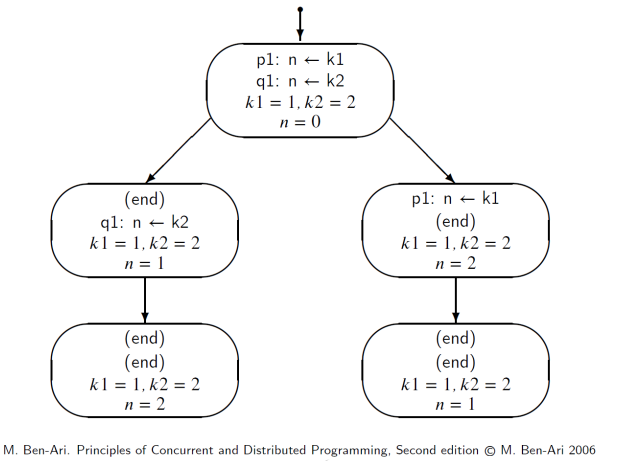
\includegraphics[scale = .45]{primoes}

\end{multicols}
...infatti un comando di assegnamento è generalmente trasformato in più di un'istruzione:
\[ \texttt{n = k + 1} \implies \begin{aligned}
                                &\texttt{load \,\,R1, k}\\
                                &\texttt{add \quad R1, \#1}\\
                                &\texttt{store R1, n}
                               \end{aligned}
 \]
 
 \newpage
Anche analizzando il primo esempio \textbf{senza l'assunzione di atomicità}, il comportamento del programma rimane però lo stesso, dato che gli unici interleaving possibili sono le permutazioni di:
\begin{center}
 
\texttt{load R1, k1} $\to$ \texttt{store R1, n} $\to$ \texttt{load R1, k2} $\to$ \texttt{store R1, n} 

\end{center}
Ed elencando tutti i casi si vede che il risultato è lo stesso.

\paragraph{E in caso di parallelismo?}

Anche se si provasse a scrivere la stessa variabile parallelamente, \textbf{l'hardware definisce un ordine}, quindi non ci sono problemi, ed il comportamento rimane lo stesso.
\subsubsection{Secondo esempio}

\[\text{Sia \texttt{int} }n \leftarrow 0 \text{ variabile condivisa:}\]
\begin{multicols}{2}
 \begin{lstlisting}
// PROCESSO P
p1: n <- n + 1\end{lstlisting}
\begin{lstlisting}
// PROCESSO Q
q1: n <- n + 1\end{lstlisting}

\end{multicols}

\textbf{In questo caso c'è effettivamente una differenza} tra il caso dell'assegnamento atomico e non:

In caso di assegnamento atomico, il valore di $n$ alla fine del programma è necessariamente 2.\medskip


Se invece si fa un'\textbf{analisi a basso livello}:

\[\text{Sia \texttt{int} }n \leftarrow 0 \text{ variabile condivisa:}\]
\begin{multicols}{2}
 \begin{lstlisting}
// PROCESSO P
p1: load  R1, n
p2: add   R1, #1
p2: store R1, n\end{lstlisting}
\begin{lstlisting}
// PROCESSO Q
q1: load  R1, n
q2: add   R1, #1
q2: store R1, n\end{lstlisting}
\end{multicols}


Queste operazioni possono essere interleaved in modo che $n$ alla fine sia 1.

\subsubsection{Simulare il comportamento a livello macchina}

Introduciamo una simulazione che ``agisce sul programma'': 

Invece di scrivere \texttt{n $\leftarrow$ n + 1} scriveremo \texttt{n $\leftarrow$ !n + 1}, che rende esplicita l'operazione di variabile.
\[ \begin{bmatrix}
    n = 0\\
    n\,\, \leftarrow \,\,!n+1
   \end{bmatrix} \longrightarrow
   \begin{bmatrix}
    n = 0\\
    n\,\, \leftarrow \,\,0+1
   \end{bmatrix} \longrightarrow
   \begin{bmatrix}
    n = 1\\
    (end)
   \end{bmatrix}
 \]

\subsection{Shared memory vs Message Passing}
Ci sono due modi per far comunicare processi tra loro:

\begin{itemize}
 \item Memoria condivisa
 \item Scambio di messaggi
\end{itemize}

\subsubsection{Memoria condivisa}
Sia $x = 0$ una variabile condivisa
 \begin{multicols}{2}
  \begin{lstlisting}
// Thread 1
producer(){
    int k = 6;
    x = fattoriale(k);
}
\end{lstlisting}
\begin{lstlisting}
//Thread 2
consumer(){
    while (x == 0) sleep(10);
    print(x);
}
\end{lstlisting}

\end{multicols}
In questo modo il thread 2 si sveglia ogni 10 secondi per controllare se il dato del producer è pronto.\newpage

Si potrebbero utilizare delle funzioni di \textbf{segnalazione} tra thread, fornite dal \textbf{runtime} del linguaggio:

 \begin{multicols}{2}
  \begin{lstlisting}
// Thread 1
producer(){
    int k = 6;
    x = fattoriale(k);
    wakeup();
}
\end{lstlisting}
\begin{lstlisting}
//Thread 2
consumer(){
    while (x == 0) sleep();
    print(x);
}
\end{lstlisting}

\end{multicols}

Dove con \textbf{sleep} il consumer si mette in attesa (non necessariamente attiva, a differenza della $sleep(t)$) e \textbf{wakeup} sveglia il consumer (il dato è pronto).


\subsubsection{Message passing}

Non utilizziamo una variabile globale, ma due funzioni \textbf{send} e \textbf{receive}:

 \begin{multicols}{2}
  \begin{lstlisting}
// Thread 1
producer(){
    int k = 6;
    x = fattoriale(k);
    send(x);
}
\end{lstlisting}
\begin{lstlisting}
//Thread 2
consumer(){
    int y = receive();
    print(y);
}
 \end{lstlisting}

 
\end{multicols}

 Il trasferimento del dato da un processo all'altro è a carico del sistema operativo.

\subsubsection{Meccanismi di sincronizzazione}
\begin{itemize}
 \item Busy waiting
 \item sleep e wakeup
 \item send e receive
 \item ...
\end{itemize}

Sono tutti meccanismi di sincronizzazione usati da \textbf{thread} e \textbf{processi}, messi a disposizione dal runtime del linguaggio (per i thread) e dal sistema operativo (per i processi).


\newpage

\section{Modello della programmazione concorrente}

\subsection{Il linguaggio}

\subsubsection{Sintassi}
\[e ::= n \,\,|\,\, e+e \,\,|\,\, !l \,\,|\,\, l := e \,\,|\,\, skip \,\,|\,\, e;e\]

Tipi: int, unit.

[\textbf{regole di tipo e semantica}: vedi slide, regole intuitive per linguaggio imperativo.]

\subsubsection{Estensione concorrente}
Estendiamo la sintassi con $e | e$, l'esecuzione concorrente di due espressioni. Chiameremo queste due espressioni \textbf{processi} (anche se si comportano in modo più simile ai \textbf{thread}), e definiamo il tipo \textbf{proc}, ``supertipo di \textbf{unit}''. 

\subsubsection{Operazioni atomiche}
Assumiamo che $+$, $!$, $:=$ e $skip$ siano atomiche.

\subsubsection{Esempio}

Eseguiamo $(l := 1 + !l) | (l := 7 + !l)$, nella memoria $\{ l \mapsto 0 \}$\smallskip

Se andiamo a disegnare il sistema di transizioni che descrive tutti i comportamenti possibili (molto grande anche per questo piccolo esempio, vd slide) notiamo che ci sono, di nuovo, vari diversi outcome, alcuni dei quali non sono ciò che ci aspettiamo! Notiamo analizzando il grafo che in questo caso tutti e soli i cammini che portano a risultati sbagliati fanno prima tutte le letture e poi tutte le scritture.\smallskip


Ci serve un meccanismo di \textbf{mutua esclusione} che ci permetta di ``rendere atomiche'' alcune parti del programma.

\subsection{Mutua esclusione}
Un \textbf{mutex} è un'entità astratta associata ad un'area di memoria da accedere in mutua esclusione.\smallskip

Estendiamo ulteriormente il linguaggio:
\[e ::= n \,\,|\,\, e+e \,\,|\,\, !l \,\,|\,\, l := e \,\,|\,\, skip \,\,|\,\, e;e \,\, | \,\,e| e \,\,|\,\, \textbf{lock }m\,\,|\,\, \textbf{unlock }m\]

dove $m \in \mathbb M$ (insieme dei \textbf{mutex}); \smallskip

Nelle regole semantiche del linguaggio aggiungiamo l'insieme dei Mutex [vd slide]; la semantica intuitiva è come segue:

\begin{itemize}
 \item Se nessuno sta accedendo all'area di memoria protetta dal mutex (i.e. se \textbf{nessuno ha ancora interagito con il mutex} oppure \textbf{l'ultima interazione con il mutex è stata una unlock}) allora il thread che chiama la \textbf{lock} procede; 
 \item Se qualcuno sta accedendo all'area di memoria (i.e. \textbf{ultima interazione = lock}) allora il thread che chiama la lock si mette in attesa che chi ha chiamato la \textbf{lock} chiami l'\textbf{unlock}.
\end{itemize}


\subsubsection{Uso dei mutex}
Il programma di prima può essere riscritto come segue:
\[ e = (\textbf{lock } m; l := 1+!l; \textbf{unlock }m) | (e = \textbf{lock } m; l := 7+!l; \textbf{unlock }m) \]

In questo modo eliminiamo la possibilità di fare tutte le letture prima delle scritture, ed otteniamo il risultato corretto: \textbf{gli assegnamenti sono eseguiti come se fossero atomici}.
\newpage
\subsubsection{Coarse-grained vs Fine-grained locking}

\begin{itemize}
 \item Strategia \textbf{coarse-grained}: un mutex per tutte le locazioni di memoria, e.g.
 
 \[ \textbf{lock }m\,\,;\,\, l_1 := 1 \,\,+\,\, !l_2 \,\,;\,\, \textbf{unlock }m \]
 
 \paragraph{Caratteristiche:} Meno lavoro al singolo thread (una sola lock), ma concorrenzza ridotta
 
 \item Strategia \textbf{fine-grained}: un mutex diverso per ogni locazione di memoria
 
  
 \[ \textbf{lock }m_1;\textbf{lock }m_2\,\,;\,\, l_1 := 1 \,\,+\,\, !l_2 \,\,;\,\, \textbf{unlock }m_1; \textbf{unlock }m_2 \]
 \paragraph{Caratteristiche:} Preferibili per la maggiore concorrenza, ma \textbf{hanno un problema}...
\end{itemize}

\[\begin{aligned}
e =&\,\,  (\textbf{lock }m_1;\textbf{lock }m_2\,\,;\,\, l_1 := !l_2 \,\,;\,\, \textbf{unlock }m_1; \textbf{unlock }m_2) \\
 |&\,\, (\textbf{lock }m_1;\textbf{lock }m_2\,\,;\,\, l_2 := !l_1 \,\,;\,\, \textbf{unlock }m_1; \textbf{unlock }m_2) 
\end{aligned}\]\smallskip


Un'analisi del sistema di transizioni ci porta a scoprire che \textbf{esistono ordini di esecuzione tali che il programma si blocca}, perché i mutex si aspettano a vicenda. \smallskip

Questa situazione prende il nome di \textbf{deadlock}.

\subsubsection{Metodi per evitare il deadlock}


\begin{itemize}
 \item \textbf{Deadlock prevention}: si stabiliscono regole controllabili staticamente che garantiscano che i deadlock non possano verificarsi.
 \item \textbf{Deadlock avoidance}: Il supporto a runtime si accorge che il programma sta per andare in deadlock ed interviene cambiando l'ordine di esecuzione dei thread.
 
 \item \textbf{Deadlock recovery}: Il programma viene lasciato libero di andare in deadlock, ma se ciò avviene il runtime del linguaggio se ne accorge ed interviene per ripristinare uno stato senza deadlock.
\end{itemize}
\subsubsection{Esempio di deadlock prevention: Two-Phase Locking}

Il locking avviene in due fasi: 

\begin{itemize}
 \item Una fase ``ascendente'' in cui si eseguono le lock 
 \item Una fase ``discendente'' in cui si eseguono le unlock, nell'ordine \textbf{opposto} rispetto a quello delle lock.
\end{itemize}

Applicando tale disciplina al programma di prima si ottiene:
\[\begin{aligned}
e =&\,\,  (\textbf{lock }m_1;\textbf{lock }m_2\,\,;\,\, l_1 := !l_2 \,\,;\,\, \textbf{unlock }m_2; \textbf{unlock }m_1) \\
 |&\,\, (\textbf{lock }m_1;\textbf{lock }m_2\,\,;\,\, l_2 := !l_1 \,\,;\,\, \textbf{unlock }m_2; \textbf{unlock }m_1) 
\end{aligned}\]
Che non può andare in deadlock.

\newpage

\section{Costrutti di concorrenza nei linguaggi di alto livello}

\subsection{Java}
In Java i thread hanno ognuno il proprio stack ma lo \textbf{heap condiviso} (shared memory).

\subsubsection{Creare thread in Java}

\begin{lstlisting}
 class Hello extends Thread{
    public void run() {
        System.out.println("Hello Thread!");
    }
 }
 
 class Main{
    public static void main(String[] args){
        Thread t = new Hello();
        t.start();                          // NON RUN!!
    }
 }
\end{lstlisting}
 Si noti che si chiama il metodo \texttt{start}, e non il metodo \texttt{run}! Chiamare quest'ultimo accederebbe al metodo della classe, facendo esecuzione sequenziale, mentre chiamare \texttt{start} crea il nuovo thread.\smallskip
 
 Un altro modo di creare un thread è il seguente:
 
 \begin{lstlisting}
 class HelloRunnable implements Runnable{
    public void run() {
        System.out.println("Hello Thread!");
    }
 }
 
 class Main{
    public static void main(String[] args){
        Runnable r = new HelloRunnable();
        Thread t = new Thread(r);
        t.start();
    }
 }
 \end{lstlisting}
In questo modo ad uno stesso thread si possono passare diversi runnable da eseguire.\smallskip

Altro modo: classe anonima:
\begin{lstlisting}
 class Main{
    public static void main(String[] args){
        Runnable r = new Runnable(){
            public void run() {
                System.out.println("Hello Thread!");
            }
        };
        Thread t = new Thread(r);
        t.start();
    }
 }
\end{lstlisting}

Inoltre, si può usare una \textbf{lambda espressione}, utile per creare oggetti con un solo metodo:
\begin{lstlisting}
 class Main{
    public static void main(String[] args){
        Runnable r = 
            () -> {System.out.println("Hello Thread!"); };
            
        Thread t = new Thread(r);
        t.start();
    }
 }
\end{lstlisting}


\subsubsection{Meccanismi di sincronizzazione}
Un primo meccanismo di sincronizzazione può essere un metodo della classe che implementa Thread, chiamato dal main (l'oggetto di quella classe è comunque visibile al main, shared memory) che scrive su una variabile (e.g. un booleano) usata dal thread per comunicare un evento 

[vd esempio Timer delle slide].\smallskip

Questo può andar bene quando tutte le interazioni tra Thread vanno in una sola direzione, o quando non ci sono interazioni, ma non sempre.\medskip

Per \textbf{eseguire due metodi della stessa classe in mutua esclusione} si utilizza il modificatore \textbf{synchronized}:

\begin{lstlisting}
...
public synchronized void incr() {n=n+1;}
public synchronized void decr() {n=n-1;}
...
\end{lstlisting}
Problema: il modificatore synchronized è \textbf{coarse grained}, cioè esegue in mutua esclusione gli interi metodi! Per un approccio più fine-grained, si usa:


\begin{lstlisting}
...
 if (val%2==0) { synchronized (this) { pari = pari+1; } }
...
\end{lstlisting}

Dove \textbf{this} è usato come ``oggetto che contiene la mutex''.\smallskip

In Java ogni oggetto contiene una mutex, quindi possiamo utilizzare un qualsiasi oggetto, anche \textbf{this}.\smallskip

Bisogna però stare attenti, quando si usano strategie di locking coarse-grained, a non finire in deadlock (usando tecniche come il two phase locking).
\subsubsection{Concorrenza nelle Collections}

Alcune collections hanno metodi synchronized: in particolare \textbf{Vector} e \textbf{HashTable}. Gli altri non ne hanno, ma la classe \textbf{Collections} mette a disposizione metodi che trasformano classi non synchronized in synchronized, come \texttt{Collections.synchronizedList}, che prende come argomento un oggetto di una qualsiasi classe che implementa \texttt{List}.

\subsection{Javascript}
Javascript usa \texttt{async} per definire una funzione che è eseguita senza interrompere il resto del codice (eseguita quindi su un nuovo thread), ed \texttt{await} per far attendere la fine dell'esecuzione di una funzione \texttt{async}. Se si passa alla funzione asincrona una funzione \texttt{callback}, la si può far chiamare alla fine dell'esecuzione.

\subsection{Go}
Prevede un costrutto \texttt{go} per definire funzioni asincrone (\textbf{goroutines}); le funzioni si sincronizzano \textbf{scambiandosi messaggi su canali}: \texttt{c <- 1} manda il segnale 1 sul canale, e \texttt{<-c} attende di ricevere.

\subsection{Erlang}
In Erlang \texttt{tutto è un processo}, ossia una \textbf{componente in esecuzione concorrente} con \texttt{memoria separata} dagli altri: \textbf{no memoria condivisa}, solo \textbf{scambio di messaggi}.

\begin{itemize}
 \item \texttt{spawn} avvia un nuovo processo
 \item \texttt{dest ! msg} invia il messaggio \textbf{msg} al processo \textbf{dest} (invio non bloccante)
 \item \texttt{receive} mette il programma in ascolto per uno o più messaggi. (receive bloccante)
\end{itemize}


\end{document}
